\documentclass[11pt,a4paper]{article}
\usepackage{float}
\usepackage[utf8]{inputenc}
\usepackage[left=2cm,right=2cm,text={18cm,24cm},top=2cm]{geometry}
\usepackage[english]{babel}
\usepackage{graphicx}
\usepackage{verbatim}
\usepackage{fancyvrb}
\usepackage{svg}
\usepackage{hyperref}
\usepackage{tabto}
\usepackage{rotating}
\usepackage{url}
\usepackage{indentfirst}
\usepackage{hyperref}


\renewcommand{\familydefault}{\sfdefault}

\begin{document}
\begin{titlepage}
	\begin{center}
		% FIT logo
		
\includegraphics[scale=0.5]{fit.pdf} \\
		
		\vspace{3cm}

  		\Large{
			IMS 2023/24 \\
		}

      \vspace{3cm}
    
		\Huge{
			\textbf{
				Simulation study} \\
    }
		\vspace{0.5cm}
        \huge {
        Model of a ski-resort
        }

        \vspace{3cm}
                                
		\Large{}
		\today{}
				
		\vspace{2cm}
  
		\begin{tabular}{l l l}
            Matyáš Strelec & \texttt{xstrel03} \\
			Ivan Chodák     & \texttt{xchoda00}  \\
		\end{tabular}
	\end{center}
    \normalsize{}
 \end{titlepage}

\pagebreak{}

\tableofcontents

\pagebreak{}

\section{Introduction}
This documentation describes a simulation \cite[slide 8]{slides} of the Czech Ski resort Říčky\cite{ricky}. In it, we represent the two main lifts, one t-bar lift supporting up to two passengers and one six-seater lift with up to six passengers at one time, three slopes with each having different difficulty, length, and time it takes to ski down it, refreshment breaks skier takes, and a way for skiers to enter and leave the ski resort via the car parking or by the shuttle bus.  \newline
We aim to study the time spent in the queues for each of the lifts depending on the different skier loads the ski center can experience and if the current infrastructure suits the ski resort's capabilities.
\subsection{Authors and data sources}
The authors of this study and research are Strelec Matyáš and Chodák Ivan. \newline
The entry data for our work were based on multiple sources. We have sourced the primary data about the resort from its official website\cite{ricky}, performed hands-on research regarding the lift speed, and drew an educated guess regarding the number of skiers in the resort based on the alleged maximal capacity \cite{stavebniserver} and the possible options of entering the system.

\subsection{Project validity}
We have verified the validity of the model \cite[slide 37]{slides} by the comparison of the behavior of the final model \cite[slide 47]{slides} and the modeled system \cite[slide 7]{slides}. The skier numbers were validated by calculating the maximum possible input of the skiers entering our system and cross-referencing it with the maximum possible capacity. Most of the skiers would enter the system around 9:30 applying normal distribution \cite[slide 93]{slides} with the standard deviation being half an hour. The skiers stop entering and start leaving the system around noon creating a two-hour window where the system both gains and loses skiers. Both the peak time for incoming skiers and the time window of their stay were based on many personal observations by both authors. We have validated the speed of the lifts by cross-referencing the data from the official website and information obtained by consulting a ski lift operator operating a similar lift in all relevant terms such as capacity, length, and speed. \newline We have observed the behavior and results of the model under different skier loads and drew conclusions based on the ratio of average wait time in given queues and the number of skiers in the system.

\section{Analysis of the topic, methods, and technologies used}
% 15% 2h 35% 4h a 50% 8h 
The ski resort is operating daily during the opening hours of 8:00-16:00 thus 8 hours. The skiers can enter the resort either by their car or a shuttle bus. There is a parking lot with a capacity of 300 cars. The incoming skier is assumed to be one of 3 categories based on their expected skiing time. Those are the short stay of around 2 hours, the medium stay of around 4 hours, and the long stay of around 8 hours. Parallel to cars coming and leaving there is also a shuttle bus coming from 7:00-14:00 in intervals based on the buses assigned according to the expected load for the day. The shuttle bus delivers a given number of skiers based on the current load and according to the same criteria of skiers' stay as with cars. From 12:00-16:00, the shuttle buses start to leave based on the same logic as when they bring skiers but in a shorter time frame. After the ski resort closes, all the remaining parked cars take their passengers and leave. The left-over skiers are taken away at the end of the day by shuttle buses with corresponding capacity. \newline
The skiers in the resort can either decide to ski or to go eat. The eat option works in two modes. Normal and lunch mode. In normal mode, there is only one option of short refreshment available. During the 11:00-13:00 the other long refreshment option becomes available offering a lunch that takes longer. The skier then again chooses a lift to the top of the mountain or decides to leave if they are done according to their endurance. If the skier goes skiing, he first picks which lift to take and joins the appropriate queue. He waits until he is serviced by the lift and delivered to the top station. At the top, he picks one of the 3 available slopes to ski on and goes down the chosen slope arriving at at the bottom station where he again decides whether to leave or stay in the resort. \newline
Thus we describe all the necessary aspects of the system that are of interest to us in this work and needed for creating different scenarios and drawing conclusions from them.
\subsection{Methods used}
We have created the simulation using the C++ language with the support of the SimLib library. C++ due to its support of Object Oriented programming allowing us to define interactions between respective entities. The SimLib library was chosen due to its ability to provide the majority of necessary implementation modules needed to represent and simulate our model giving us more freedom to focus on the logic of the system and experimenting instead of implementing the basics.

\subsection{Technologies used}
For the creation of the simulation, the Simlib library and the C++ language were used. For the correct usage of the Simlib library, sample source codes were utilized.
\footnote{Simlib examples: \url{http://www.fit.vutbr.cz/~peringer/SIMLIB/examples/}}
The official version of the Simlib library was used.
\footnote{Simlib documentation: \url{http://www.fit.vutbr.cz/~peringer/SIMLIB}}
Standard C++ libraries were used as well. \footnote{C++ documentation: \url{http://en.cppreference.com/w/}}.

\section{Concept}
In this section, we will go over the design for the conceptual/abstract model \cite[slide 48]{slides} on a system that can be represented by the queuing model(SHO) \cite[slide 139]{slides}. The model should represent the important parts of the system and their behaviors. Thus we chose to model skiers as individual processes that are being serviced by different service lines. These service lines represent ski lifts. The processes can have different behaviors.


\subsection{Method of expressing the model}
Model is represented via Petri net \cite[slide 129]{slides} and is included in the attachment \ref{appendix:petrinet}. The model is composed of different service lines \cite[slide 149]{slides}, queues \cite[slide 141]{slides}, events\cite[slide 166]{slides}, and processes\cite[slide 139]{slides}.
The states and transitions between them describe different relations and flows making up the net. It describes two main portions of the system, the parking and the resort, interacting together through one common base state the lower lift station (referenced to from now as a base state). The parking portion handles the car generator, parking capacity control, skier spawning and their removal from the system. It also takes care of the shuttle bus in a similar manner without the need to control the parking capacity. \newline
The resort simulates the behavior of the skier during his stay allowing him to make decisions altering his state in the system. 

\subsection{The description of the conceptual model}
The lifts are running for 8 hours a day from 8:00 to 16:00. The skiers arrive by car which tries to find a parking space. If it were unsuccessful due to the full capacity it leaves. The cars arrive mostly between 8:00 and 12:00 with the normal distribution of 9:30 and a standard deviation of 30 minutes simulating the peak entry load by car. If parked, it spawns skiers accordingly. Each car spawns 1 to 5, based on normal distribution with mean 3 and standard deviation 1, skiers of the stay endurance quality. By this logic cars can arrive before the lifts start. In this case, the skiers just wait for lifts to start, simulating the initial load of the early skiers. The car remembers the amount of skiers which each stay in the system for a duration based on a normal distribution of their 
respective skill. The short stay is based on the middle value of 2 hours, the medium stay of 4 hours, and the long stay of 8 hours. After the given period is up or when the ski resort closes they get ready to leave and wait until their car can leave with all the occupants it came in with. The buses come in based on uniform distribution\cite[str. 89]{slides} from 7:00 to 14:00 with a number of buses per day set by a variable. They leave based on the same criteria as they arrived in but in a shorter time period. They each take away their respective capacity with extra shuttle buses being present at the end of the day to transport all the remaining skiers that didn't come by car. \newline
The resort has a control base state that is used for input and output of the skiers in the resort connected to the parking which controls these numbers. Skier that stays moves to a next state where he decides if he is going to ski or eat. If he goes to eat he can pick from a short break or a long break if the lunch is being served both taking their time based on normal distribution with base of 15 minutes for the and 60 minutes for the long break with standard deviation being 15 minutes. He then returns back to the base state where he either leaves or goes to the next decision-making state again. If he decides to ski, he picks which lift to take and joins its queue. Once he got to the lift he is transported to the top of the hill. There he picks which slope to ski on and is then added to the shared base state after the time it takes for the given slope runs out. Each slope has a time it takes to get to the bottom based on normal distribution with bases of 7.3 minutes for the red, 8.5 minutes for the blue, and 6.1 minutes for the  black with standard deviations being 30 seconds for the red, 60 seconds for the blue, and 40 seconds for the black.  
\section{Architecture of the simulation model}
When running the simulation model \cite[slide 44]{slides}, the model is simulated with the given parameters. If the user does not give any parameters, the default ones are used. At the end of the run the simulation, statistics are written to standard output. There are statistics for the two lift queues with their average length of people and waiting times, and the parking lot with average, minimal, and maximal capacity used. Last, there are information about the skiers that is used in the experiments, namely the total number of skiers that day, and average values for time spent in queues, on lifts and skiing. One time unit equals one second.

The simulation starts at 6AM and ends at 6PM. Cars, buses and people arriving on foot are generated form the amounts in arguments. The lifts are set to activate on the opening time, then the simulation is ran. 
\subsection{Mapping the abstract model to the simulation model}
The skier is implemented as a process, which after some waiting goes to queue in the queue of the lift that they pick. The process is passivated and waits to be activated by the queue process when it reaches top of the lift. Then, the skiing time is implemented by waiting. The skier has some timeout, which will trigger if their Skipass time runs out, or they are removed from the queue at the closing time. Then, they decide to leave, which is implemented using another queue.

The chairlifts are implemented as separate processes. The interval of the gates opening is calculated, every interval the lift takes some skiers waiting in the queue. The number of skiers is decided randomly, by the rate of occupancy of the lift. If the time reaches the closing time, skiers are taken out of the queue.

The cars and buses are implemented as processes. After being activated, they wait for some pseudo-random time to simulate arrivals. The car parks in the car park (if there are free spots) or leaves (if there are none). The car creates 1-6 skiers, the bus creates 40 people with normal distribution and deviation of 10. Then, the processes wait until the skiers are finished and in the queue ready to leave. Then, the skiers are terminated and cars or buses leave the system.

\subsection{Running the simulation model}
To compile, use the \verb|make| command, or to run with default parameters, use \verb|make run|. The default parameters are described in the section 5.

To run manually, run \verb|./main {params}|.

The parameters, which can be used on the command line are following:
\begin{itemize}
    \item \verb|cars|: cars per day, default 200
    \item \verb|buses|: buses per day, default 4
    \item \verb|tbarpow|: T-bar power (0-100), default 75
    \item \verb|chairpow|: chairlift power (0-100), default 85
    \item \verb|parking|: capacity of the parking lot, default 300
\end{itemize}

\section{The nature of simulation experiments and their course}
One of the first steps was to prove the validity of our system. We then created three load scenarios each representing low load, medium load, and high load respectively. After running each load preset given amount of times we gained the average for the following values: wait time for each lift, the overall wait time in the queue during their stay, the overall time spent riding the lift, the overall time spent skiing, and the ratio of skiing to waiting based on which we drew most conclusions. We also gain other statistics that might be interesting for individual simulations. 

\subsection{Procedure of experimentation}
The simulation was run with four different test cases each being 14 times simulating 2 weeks at given capacity. Based on the average of the obtained values we evaluated each test case and dew conclusions.

\subsection{Documentation of individual experiments}
\subsubsection{Validating the created model}
We have done field research in a resort with similar properties seeking to find the ratio of skiing to waiting + being transported by the lift. Based on the collected data for the duration for 3.5hours resulting in 17 rides, 42 minutes of skiing, 1 hour 6 minutes being spent on the lift and 1 hour 46minutes being spent waiting (this includes roughly 40-minute refreshment break which was not taken into account when calculating aimed average), we concluded the ratio (time skiing : time in queue + on the lift) should be 1:2 rounded to indicate a happy skier with a good amount of skiing done relative to his wait time. 
For the validation test we have tried simulating a similar load to the real-life testing scenario.

\begin{table}[H]
		\centering
		\begin{tabular}{|r|r|r|r|r|}
			\hline
			\textbf{Cars/day} &\textbf{Buses/day} & \textbf{T-bar power[\%]} 
				& \textbf{Chairlift power[\%]} & \textbf{Parking capacity} \\ \hline

			 200 & 4 & 75 & 85& 300\\ \hline
		\end{tabular}

		\caption{Parameters 1}
		\label{table:param1}
	\end{table}


\begin{table}[H]
    \centering
    \begin{tabular}{|r|r|r|r|r|r|r|}
        \hline
        \textbf{All skiers} &\textbf{Max rides} & \textbf{Avg rides} 
            & Time skiing[H] & Time waiting[H] & Time in lift[H]
            & \textbf{The ratio} \\ \hline

        865.21 & 34.64 & 15.38 & 2.15 & 1.73 & 1.19 & 0.691  \\ \hline
    \end{tabular}

    \caption{Experiment 1}
    \label{table:experiment1}
\end{table}

\subsubsection{Testing low load}
We are testing a low load to verify that the ratio will better in response to fewer skiers in the systems thus producing better wait time ratio. At these capacities, the skiers are nearly unaffected by the wait time.
\begin{table}[H]
		\centering
		\begin{tabular}{|r|r|r|r|r|}
			\hline
			\textbf{Cars/day} &\textbf{Buses/day} & \textbf{T-bar power[\%]} 
				& \textbf{Chairlift power[\%]} & \textbf{Parking capacity} \\ \hline

			 100 & 2 & 75 & 85& 300\\ \hline
		\end{tabular}

		\caption{Parameters 2}
		\label{table:param2}
	\end{table}


\begin{table}[H]
    \centering
    \begin{tabular}{|r|r|r|r|r|r|r|}
        \hline
        \textbf{All skiers} &\textbf{Max rides} & \textbf{Avg rides} 
            & Time skiing[H] & Time waiting[H] & Time in lift[H]
            & \textbf{The ratio} \\ \hline

        423.71 & 47.21 & 23.31 & 3.37 & 0.08 & 1.81 & 1.73  \\ \hline
    \end{tabular}

    \caption{Experiment 2}
    \label{table:experiment2}
\end{table}

\subsubsection{Testing medium load}
Here we are simulating the average load on the ski resort as a reference value. 
\begin{table}[H]
    \centering
    \begin{tabular}{|r|r|r|r|r|}
        \hline
        \textbf{Cars/day} &\textbf{Buses/day} & \textbf{T-bar power[\%]} 
            & \textbf{Chairlift power[\%]} & \textbf{Parking capacity} \\ \hline

         180 & 4 & 75 & 85& 300\\ \hline
    \end{tabular}

    \caption{Parameters 3}
    \label{table:param3}
\end{table}

\begin{table}[H]
    \centering
    \begin{tabular}{|r|r|r|r|r|r|r|}
        \hline
        \textbf{All skiers} &\textbf{Max rides} & \textbf{Avg rides} 
            & Time skiing[H] & Time waiting[H] & Time in lift[H]
            & \textbf{The ratio} \\ \hline

        791.07 & 36.57 & 16.29 & 2.31 & 1.44 & 1.28 & 0.85  \\ \hline
    \end{tabular}

    \caption{Experiment 3}
    \label{table:experiment3}
\end{table}

\subsubsection{Testing high load}
Testing a high volume of skiers in the system and how it worsens the waiting ratio.
\begin{table}[H]
		\centering
		\begin{tabular}{|r|r|r|r|r|}
			\hline
			\textbf{Cars/day} &\textbf{Buses/day} & \textbf{T-bar power[\%]} 
				& \textbf{Chairlift power[\%]} & \textbf{Parking capacity} \\ \hline

			 400 & 8 & 75 & 85& 300\\ \hline
		\end{tabular}

		\caption{Parameters 4}
		\label{table:param4}
	\end{table}


\begin{table}[H]
    \centering
    \begin{tabular}{|r|r|r|r|r|r|r|}
        \hline
        \textbf{All skiers} &\textbf{Max rides} & \textbf{Avg rides} 
            & Time skiing[H] & Time waiting[H] & Time in lift[H]
            & \textbf{The ratio} \\ \hline

        1436.00 & 24.43 & 10.07 & 2.86 & 1.73 & 0.76 & 0.38  \\ \hline
    \end{tabular}

    \caption{Experiment 4}
    \label{table:experiment4}
\end{table}

\subsubsection{Testing high load}
Testing a high volume of skiers in the system and how it worsens the waiting ratio.
\begin{table}[H]
		\centering
		\begin{tabular}{|r|r|r|r|r|}
			\hline
			\textbf{Cars/day} &\textbf{Buses/day} & \textbf{T-bar power[\%]} 
				& \textbf{Chairlift power[\%]} & \textbf{Parking capacity} \\ \hline

			 400 & 8 & 75 & 85& 300\\ \hline
		\end{tabular}

		\caption{Parameters 5}
		\label{table:param5}
	\end{table}


\begin{table}[H]
    \centering
    \begin{tabular}{|r|r|r|r|r|r|r|}
        \hline
        \textbf{All skiers} &\textbf{Max rides} & \textbf{Avg rides} 
            & Time skiing[H] & Time waiting[H] & Time in lift[H]
            & \textbf{The ratio} \\ \hline

        1436.00 & 24.43 & 10.07 & 2.86 & 1.73 & 0.76 & 0.38  \\ \hline
    \end{tabular}

    \caption{Experiment 5}
    \label{table:experiment5}
\end{table}


\subsubsection{Testing higher load with current parking}
Testing a higher number of cars with the current parking capacity.
\begin{table}[H]
		\centering
		\begin{tabular}{|r|r|r|r|r|}
			\hline
			\textbf{Cars/day} &\textbf{Buses/day} & \textbf{T-bar power[\%]} 
				& \textbf{Chairlift power[\%]} & \textbf{Parking capacity} \\ \hline

			 500 & 8 & 75 & 85& 300\\ \hline
		\end{tabular}

		\caption{Parameters 6}
		\label{table:param6}
	\end{table}


\begin{table}[H]
    \centering
    \begin{tabular}{|r|r|r|r|r|r|r|}
        \hline
        \textbf{All skiers} &\textbf{Max rides} & \textbf{Avg rides} 
            & Time skiing[H] & Time waiting[H] & Time in lift[H]
            & \textbf{The ratio} \\ \hline

        1464.00 & 23.86 & 10.17 & 2.94 & 0.76 & 1.37 & 0.37  \\ \hline
    \end{tabular}

    \caption{Experiment 6}
    \label{table:experiment6}
\end{table}


\subsubsection{Testing higher load with doubled parking}
Testing a higher number of cars with the doubled parking capacity and observing how it affects the system.
\begin{table}[H]
		\centering
		\begin{tabular}{|r|r|r|r|r|}
			\hline
			\textbf{Cars/day} &\textbf{Buses/day} & \textbf{T-bar power[\%]} 
				& \textbf{Chairlift power[\%]} & \textbf{Parking capacity} \\ \hline

			 500 & 8 & 75 & 85& 600\\ \hline
		\end{tabular}

		\caption{Parameters 7}
		\label{table:param7}
	\end{table}


\begin{table}[H]
    \centering
    \begin{tabular}{|r|r|r|r|r|r|r|}
        \hline
        \textbf{All skiers} &\textbf{Max rides} & \textbf{Avg rides} 
            & Time skiing[H] & Time waiting[H] & Time in lift[H]
            & \textbf{The ratio} \\ \hline

        2086.14 & 20.00 & 7.25 & 3.48 & 0.53 & 0.96 & 0.24  \\ \hline 
    \end{tabular}

    \caption{Experiment 7}
    \label{table:experiment7}
\end{table}

\subsection{Experiments conclusions}
We have run 98 simulations in 7 different test case settings. During this period we came to the conclusion the original model is valid and can produce useful data showing different loads on the system. We also concluded that the current resort and its infrastructure are the right match for their respective capacities. However, at higher loads the wait time ratio is getting worse thus don't recommend running the resort at those capacities due to the worsening satisfaction of skiers.
We also tried doubling the parking capacity however the system could not support such a load increase. In this experiment, the doubled capacity actually worsened the ratio of skiing to waiting, therefore, the capacity of the lifts must be increased to facilitate more cars.


\section{Summary of simulation experiments and conclusions}

Through simulation experiments conducted on the developed model, as seen in Chapter 5.2.1, its validity was verified because, under the initial parameter values of the model corresponding to the acquired real-world facts, the model behaved analogously to the real system.
The study performed on the model demonstrated that the system is designed in such a way that, under current conditions, it can effectively handle the currently designed load however the higher end of load capacity results in worsened skier satisfaction. We do not recommend expanding the parking capacity at the moment.

\pagebreak

\bibliographystyle{doc/czechiso}
\bibliography{doc/doc}

\clearpage
\appendix


\section{Petri net}
\label{appendix:petrinet}

\begin{figure}[H]
    \centering
    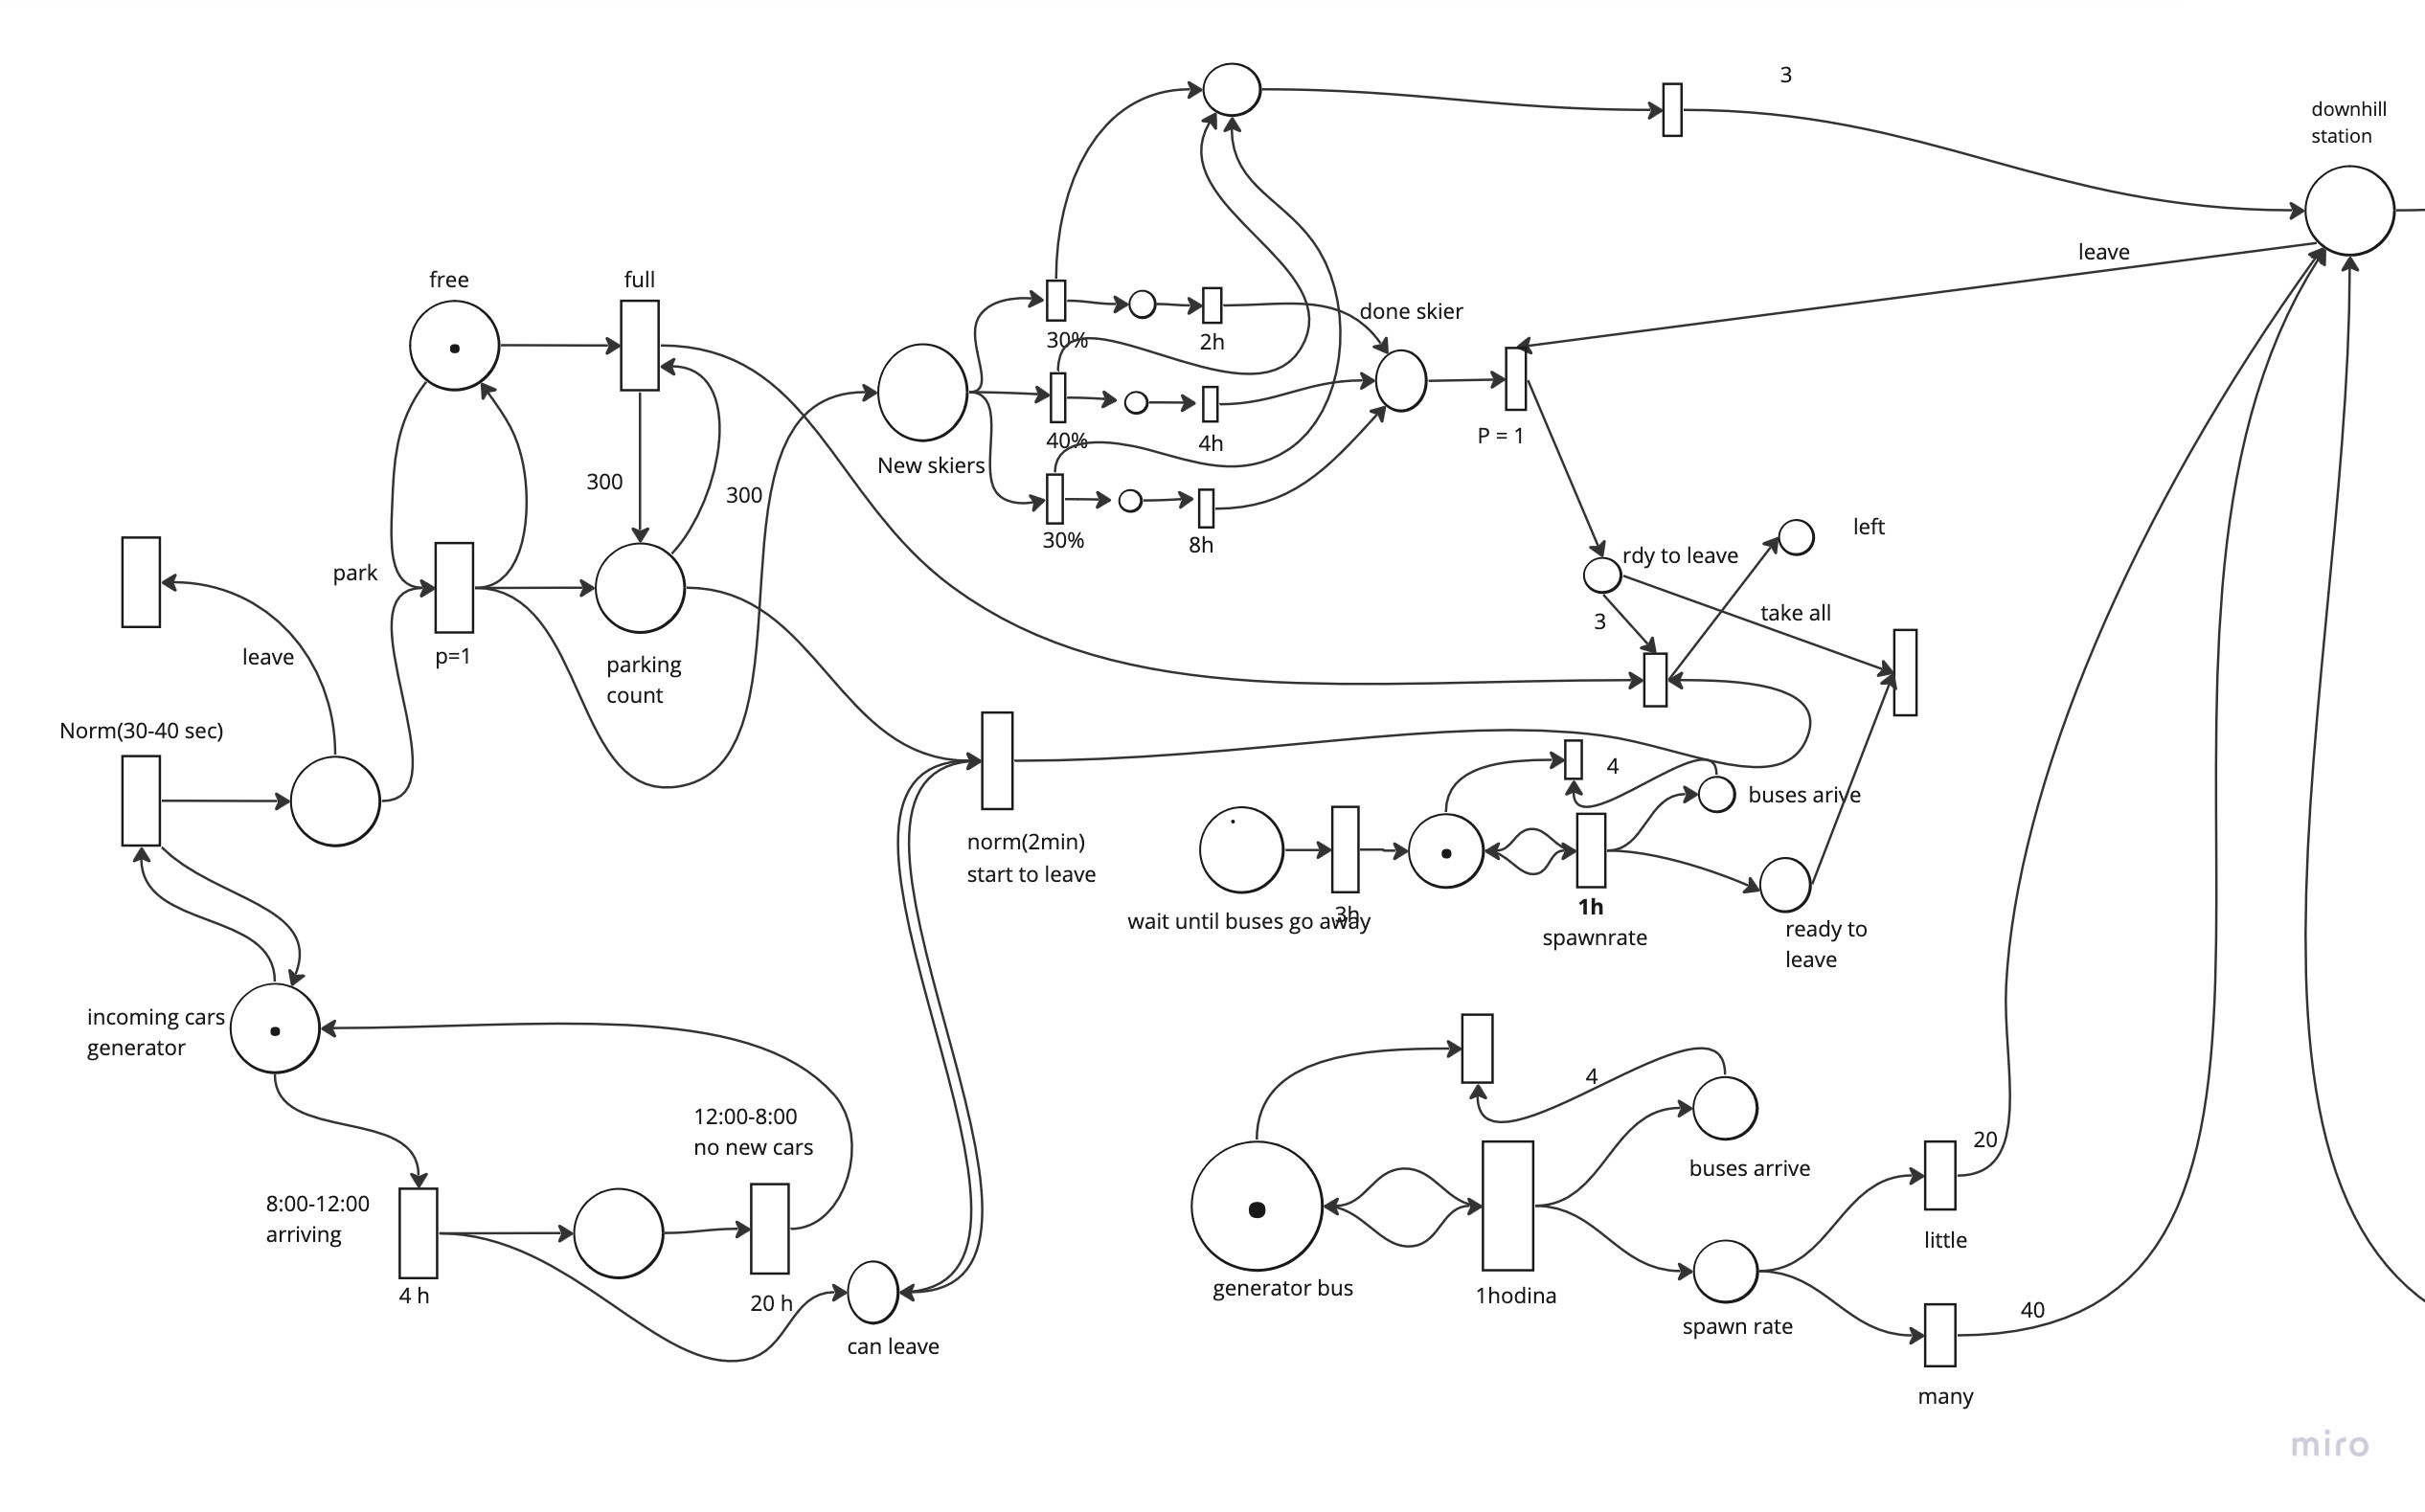
\includegraphics[width=0.85 \linewidth]{doc/petri-1.jpg}
    \caption{Petri net of incoming processes to system}
\end{figure}

 \begin{figure}[H]
    \centering
    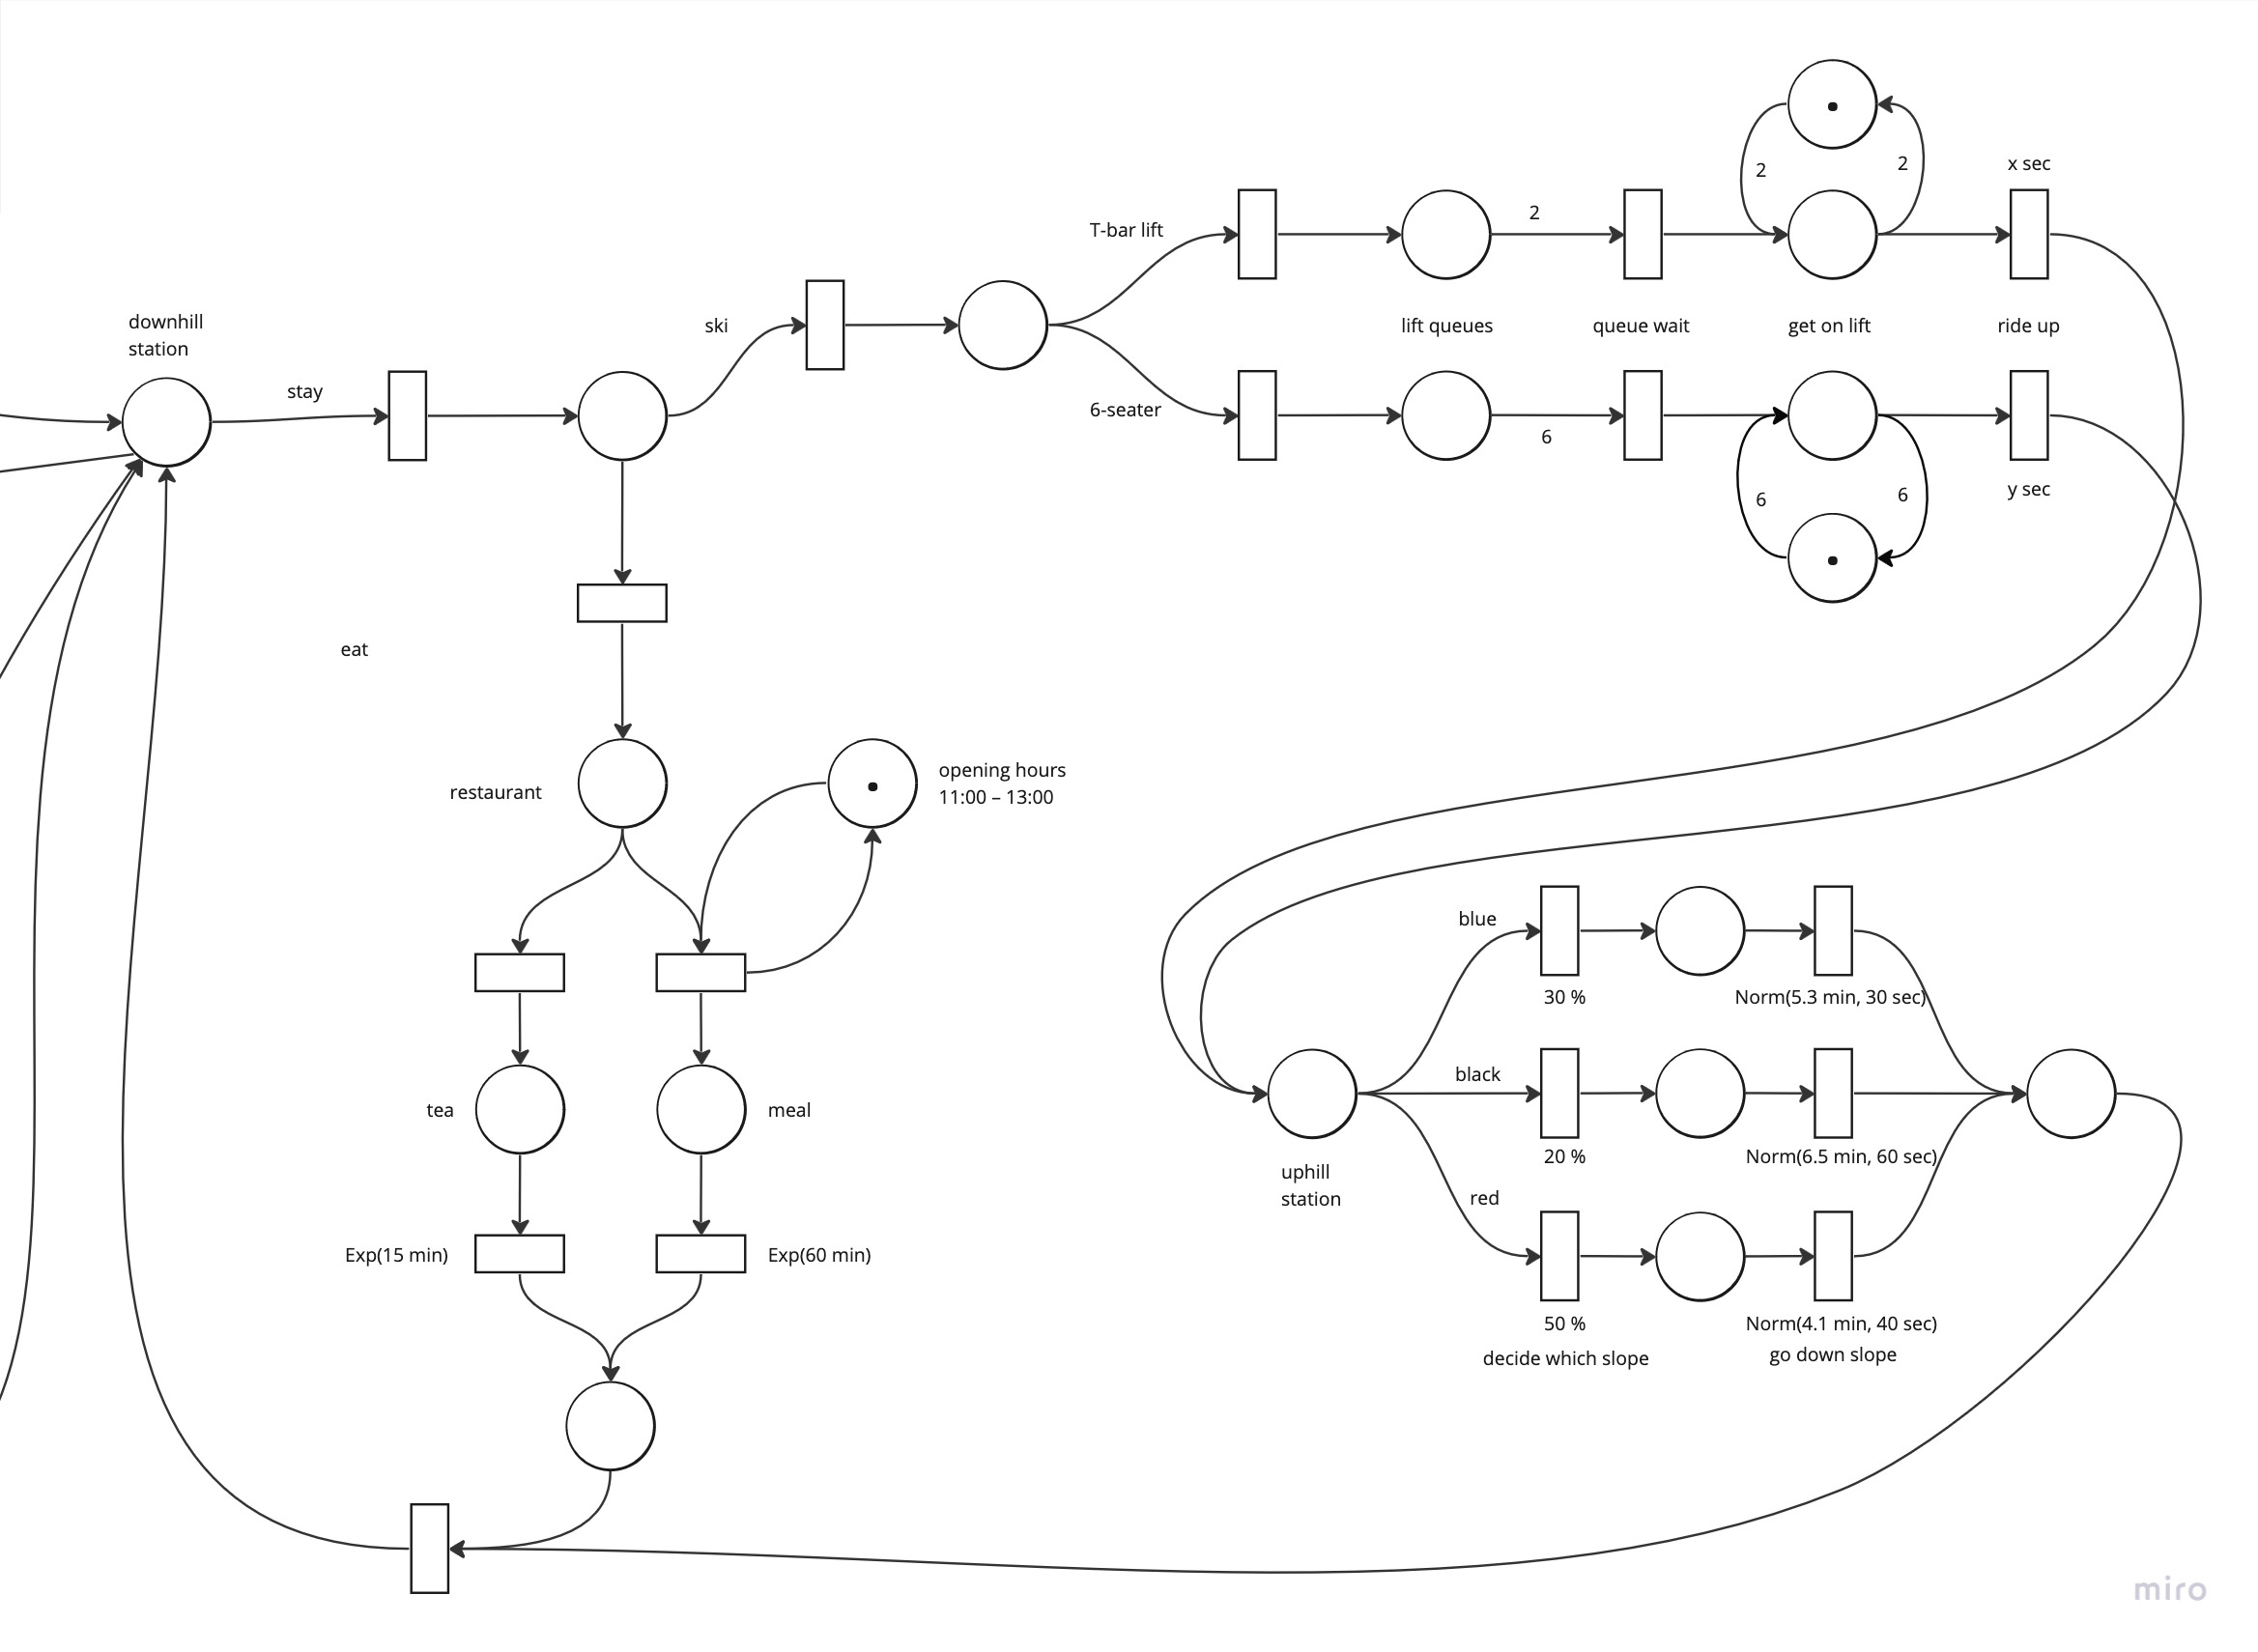
\includegraphics[width=0.85 \linewidth]{doc/petri-2.jpg}
    \caption{Petri net of skier process in system}
\end{figure}

\end{document}